%%
%% This is file `sample-sigconf.tex',
%% generated with the docstrip utility.
%%
%% The original source files were:
%%
%% samples.dtx  (with options: `all,proceedings,bibtex,sigconf')
%% 
%% IMPORTANT NOTICE:
%% 
%% For the copyright see the source file.
%% 
%% Any modified versions of this file must be renamed
%% with new filenames distinct from sample-sigconf.tex.
%% 
%% For distribution of the original source see the terms
%% for copying and modification in the file samples.dtx.
%% 
%% This generated file may be distributed as long as the
%% original source files, as listed above, are part of the
%% same distribution. (The sources need not necessarily be
%% in the same archive or directory.)
%%
%%
%% Commands for TeXCount
%TC:macro \cite [option:text,text]
%TC:macro \citep [option:text,text]
%TC:macro \citet [option:text,text]
%TC:envir table 0 1
%TC:envir table* 0 1
%TC:envir tabular [ignore] word
%TC:envir displaymath 0 word
%TC:envir math 0 word
%TC:envir comment 0 0
%%
%% The first command in your LaTeX source must be the \documentclass
%% command.
%%
%% For submission and review of your manuscript please change the
%% command to \documentclass[manuscript, screen, review]{acmart}.
%%
%% When submitting camera ready or to TAPS, please change the command
%% to \documentclass[sigconf]{acmart} or whichever template is required
%% for your publication.
%%
%%
% \documentclass[sigconf]{acmart}
\documentclass[sigconf, anonymous, review]{acmart}
%%
%% \BibTeX command to typeset BibTeX logo in the docs
\AtBeginDocument{%
  \providecommand\BibTeX{{%
    Bib\TeX}}}

%% Rights management information.  This information is sent to you
%% when you complete the rights form.  These commands have SAMPLE
%% values in them; it is your responsibility as an author to replace
%% the commands and values with those provided to you when you
%% complete the rights form.
\setcopyright{acmlicensed}
\copyrightyear{2018}
\acmYear{2018}
\acmDOI{XXXXXXX.XXXXXXX}
%% These commands are for a PROCEEDINGS abstract or paper.
\acmConference[Conference acronym 'XX]{Make sure to enter the correct
  conference title from your rights confirmation email}{June 03--05,
  2018}{Woodstock, NY}
%%
%%  Uncomment \acmBooktitle if the title of the proceedings is different
%%  from ``Proceedings of ...''!
%%
%%\acmBooktitle{Woodstock '18: ACM Symposium on Neural Gaze Detection,
%%  June 03--05, 2018, Woodstock, NY}
\acmISBN{978-1-4503-XXXX-X/2018/06}


%%
%% Submission ID.
%% Use this when submitting an article to a sponsored event. You'll
%% receive a unique submission ID from the organizers
%% of the event, and this ID should be used as the parameter to this command.
%%\acmSubmissionID{123-A56-BU3}

%%
%% For managing citations, it is recommended to use bibliography
%% files in BibTeX format.
%%
%% You can then either use BibTeX with the ACM-Reference-Format style,
%% or BibLaTeX with the acmnumeric or acmauthoryear sytles, that include
%% support for advanced citation of software artefact from the
%% biblatex-software package, also separately available on CTAN.
%%
%% Look at the sample-*-biblatex.tex files for templates showcasing
%% the biblatex styles.
%%

%%
%% The majority of ACM publications use numbered citations and
%% references.  The command \citestyle{authoryear} switches to the
%% "author year" style.
%%
%% If you are preparing content for an event
%% sponsored by ACM SIGGRAPH, you must use the "author year" style of
%% citations and references.
%% Uncommenting
%% the next command will enable that style.
%%\citestyle{acmauthoryear}


%%
%% end of the preamble, start of the body of the document source.
\begin{document}

%%
%% The "title" command has an optional parameter,
%% allowing the author to define a "short title" to be used in page headers.
\title{The Name of the Title Is Hope}

%%
%% The "author" command and its associated commands are used to define
%% the authors and their affiliations.
%% Of note is the shared affiliation of the first two authors, and the
%% "authornote" and "authornotemark" commands
%% used to denote shared contribution to the research.
\author{Ben Trovato}
\authornote{Both authors contributed equally to this research.}
\email{trovato@corporation.com}
\orcid{1234-5678-9012}
\author{G.K.M. Tobin}
\authornotemark[1]
\email{webmaster@marysville-ohio.com}
\affiliation{%
  \institution{Institute for Clarity in Documentation}
  \city{Dublin}
  \state{Ohio}
  \country{USA}
}

\author{Lars Th{\o}rv{\"a}ld}
\affiliation{%
  \institution{The Th{\o}rv{\"a}ld Group}
  \city{Hekla}
  \country{Iceland}}
\email{larst@affiliation.org}

\author{Valerie B\'eranger}
\affiliation{%
  \institution{Inria Paris-Rocquencourt}
  \city{Rocquencourt}
  \country{France}
}

\author{Aparna Patel}
\affiliation{%
 \institution{Rajiv Gandhi University}
 \city{Doimukh}
 \state{Arunachal Pradesh}
 \country{India}}

\author{Huifen Chan}
\affiliation{%
  \institution{Tsinghua University}
  \city{Haidian Qu}
  \state{Beijing Shi}
  \country{China}}

\author{Charles Palmer}
\affiliation{%
  \institution{Palmer Research Laboratories}
  \city{San Antonio}
  \state{Texas}
  \country{USA}}
\email{cpalmer@prl.com}

\author{John Smith}
\affiliation{%
  \institution{The Th{\o}rv{\"a}ld Group}
  \city{Hekla}
  \country{Iceland}}
\email{jsmith@affiliation.org}

\author{Julius P. Kumquat}
\affiliation{%
  \institution{The Kumquat Consortium}
  \city{New York}
  \country{USA}}
\email{jpkumquat@consortium.net}

%%
%% By default, the full list of authors will be used in the page
%% headers. Often, this list is too long, and will overlap
%% other information printed in the page headers. This command allows
%% the author to define a more concise list
%% of authors' names for this purpose.
\renewcommand{\shortauthors}{Trovato et al.}

%%
%% The abstract is a short summary of the work to be presented in the
%% article.
\begin{abstract}

LLM agents with web access are increasingly becoming the default for user-facing question answering. Reliable evaluation in this setting requires tests that remain unseen at train time and cannot be answered via verbatim lookup at inference. However, standard practice still relies on static benchmarks that age quickly and are vulnerable to contamination. We analyze two channels, pretraining leakage where test items appear in the pretraining data, and run-time leakage where the agent finds the exact target answer verbatim during evaluation and reports it rather than demonstrating genuine problem solving. We uncover evidence across five QA datasets for both pretraining and run-time leakage, and we show that static evaluation can overestimate capability. We introduce DynamicWebQA, a dynamic evaluation framework that constructs questions and verifiable answers at evaluation time from relevant web sources. The framework enforces multi-document grounding, records evidence chains, and offers controllable complexity through source set size, number of hops, and reasoning constraints. By generating fresh test instances, DynamicWebQA reduces memorization risk, mitigates run-time leakage, and naturally covers time-sensitive queries. 

\end{abstract}

%%
%% The code below is generated by the tool at http://dl.acm.org/ccs.cfm.
%% Please copy and paste the code instead of the example below.
%%
\begin{CCSXML}
<ccs2012>
 <concept>
  <concept_id>00000000.0000000.0000000</concept_id>
  <concept_desc>Do Not Use This Code, Generate the Correct Terms for Your Paper</concept_desc>
  <concept_significance>500</concept_significance>
 </concept>
 <concept>
  <concept_id>00000000.00000000.00000000</concept_id>
  <concept_desc>Do Not Use This Code, Generate the Correct Terms for Your Paper</concept_desc>
  <concept_significance>300</concept_significance>
 </concept>
 <concept>
  <concept_id>00000000.00000000.00000000</concept_id>
  <concept_desc>Do Not Use This Code, Generate the Correct Terms for Your Paper</concept_desc>
  <concept_significance>100</concept_significance>
 </concept>
 <concept>
  <concept_id>00000000.00000000.00000000</concept_id>
  <concept_desc>Do Not Use This Code, Generate the Correct Terms for Your Paper</concept_desc>
  <concept_significance>100</concept_significance>
 </concept>
</ccs2012>
\end{CCSXML}

\ccsdesc[500]{Do Not Use This Code~Generate the Correct Terms for Your Paper}
\ccsdesc[300]{Do Not Use This Code~Generate the Correct Terms for Your Paper}
\ccsdesc{Do Not Use This Code~Generate the Correct Terms for Your Paper}
\ccsdesc[100]{Do Not Use This Code~Generate the Correct Terms for Your Paper}

%%
%% Keywords. The author(s) should pick words that accurately describe
%% the work being presented. Separate the keywords with commas.
\keywords{Do, Not, Use, This, Code, Put, the, Correct, Terms, for,
  Your, Paper}
%% A "teaser" image appears between the author and affiliation
%% information and the body of the document, and typically spans the
%% page.


\received{20 February 2007}
\received[revised]{12 March 2009}
\received[accepted]{5 June 2009}

%%
%% This command processes the author and affiliation and title
%% information and builds the first part of the formatted document.

\maketitle

\section{Introduction}
TBD

\section{Related Work}

\subsection{Preliminaries}

\subsubsection{Benchmark Leakage}

Benchmark leakage refers to the contamination that occurs when a model has prior exposure to a benchmark's test items during pretraining, leading to inflated evaluation scores and undermining the benchmark's validity \cite{zhouDontMakeYour2023,zhuDyValDynamicEvaluation2024b}. Since most LLMs are pretrained indiscriminately on publicly available web content, there is a high likelihood that they might have encountered benchmark datasets hosted on platforms like HuggingFace, GitHub, Kaggle, and similar sites. If the base LLM used in a WebQA agent has already seen the test examples during pretraining, the evaluation effectively becomes a case of testing on the training set — severely compromising the credibility of the reported results.

\subsubsection{Dynamic Benchmarking}

Dynamic benchmarking is an emerging evaluation paradigm that generates or adapts test samples at evaluation time, so models are scored on fresh, unseen data and testset contamination is avoided \cite{zhuDyValDynamicEvaluation2024b,kielaDynabenchRethinkingBenchmarking2021a,maDynaboardEvaluationAsAServicePlatform2021,zhuDynamicEvaluationLarge2024,zhangDARGDynamicEvaluation2024,rawlesAndroidWorldDynamicBenchmarking2025}. That means the agent does not see the same test sample twice, effectively addressing issues such as LLM memorization.

\subsubsection{Evolving Information}

In this work, we refer to information that can change over time, such as the stock price of Tesla, as evolving information. Arguably, this type of content could be labeled as dynamic content or temporal content, but that might cause confusion, since we are already using the term ``dynamic'' to describe an evaluation paradigm (dynamic benchmarking), and ``temporal'' might lead readers to associate it with time-series data. To avoid such confusion, we adopt the term evolving information to specifically denote factual content that may shift over time without implying a particular format or evaluation framework.

\subsection{Related Work}

\subsubsection{Open-Domain QA and Retrieval-Augmented Agents}

Open-domain question answering traditionally involves retrieving relevant documents and extracting or generating an answer. For instance, consider DrQA \cite{chenReadingWikipediaAnswer2017a}, which combined a TF-IDF document retriever with a neural reader to answer questions using Wikipedia. Since then, large-scale datasets like Natural Questions \cite{kwiatkowskiNaturalQuestionsBenchmark2019a}, TriviaQA \cite{joshiTriviaQALargeScale2017} and HotPotQA \cite{yangHotpotQADatasetDiverse2018a} have driven progress in retrieval-based QA, with models achieving impressive in-domain accuracy. The introduction of transformer-based retrievers and readers led to substantial gains – for example, dense passage retrieval and a fusion-in-decoder reader (FiD) improved open QA by aggregating information from multiple passages \cite{izacardLeveragingPassageRetrieval2021}. More recently, the trend has shifted to retrieval-augmented generation (RAG) systems \cite{yaoReActSynergizingReasoning2023a}, which integrate retrieval into the generative process. In a RAG model, an LLM conditions on retrieved text chunks when constructing its answer, thereby injecting fresh knowledge and reducing factual errors. RAG-based approaches have become a standard for knowledge-intensive tasks, demonstrating superior factual accuracy and generality \cite{yaoReActSynergizingReasoning2023a}.

With improvements in LLM reasoning capabilities, research has shifted towards agentic frameworks where a model iteratively interacts with tools, such as search engines and knowledge graphs, to answer queries. For example, WebGPT \cite{nakanoWebGPTBrowserassistedQuestionanswering2022a} augments an LLM with the ability to issue web search queries and navigate webpages, guided by human feedback to produce high-quality answers with citations. Other works like ReAct \cite{yaoReActSynergizingReasoning2023a} combines reasoning steps with tool use, allowing the model to plan multi-step solutions (e.g. search for a fact, then use a calculator) in a single unified prompting framework. These ``LLM-as-agent'' approaches are promising because they mimic how humans gather and verify information, and they can handle more complex queries that require multi-hop reasoning or cross-referencing sources \cite{zhuLargeLanguageModels2025}. 

\subsubsection{Robustness of QA Systems}

Robustness of QA systems has garnered a lot of interest as researchers realized that high IID (in-distribution) test scores do not guarantee real-world reliability \cite{thakurBEIRHeterogenousBenchmark2021}. Prior research has examined multiple facets of robustness. One line of work looks at adversarial robustness: for example, adding misleading but irrelevant sentences to a passage can confuse models that lack true understanding \cite{jiaAdversarialExamplesEvaluating2017}. This revealed that many QA models rely on shallow cues and can be tricked by simple perturbations. In open-domain QA, models must also cope with naturally occurring distractions or errors in retrieved text. The HotpotQA dataset \cite{yangHotpotQADatasetDiverse2018a}, which requires multi-hop reasoning across multiple Wikipedia articles and includes some irrelevant paragraphs, was an early attempt to test a model's ability to stay focused on relevant facts. Dense retrievers and readers have been shown to drop in accuracy when deployed on different source distributions or domains – for instance, a model trained on Wikipedia may struggle on biomedical articles. The BEIR benchmark \cite{thakurBEIRHeterogenousBenchmark2021} quantified this by evaluating retrieval models on 18 heterogeneous IR tasks: no single model performed uniformly well across all domains, highlighting generalization gaps.

Another crucial aspect is temporal robustness. QA models quickly become outdated as world knowledge changes. To address this, temporal benchmarks have been proposed to evaluate systems on questions about current events or facts that change over time. RealTime QA \cite{kasaiRealTimeQAWhats2024}, for example, continually releases new questions (on a weekly basis) about recent news and evaluates systems' ability to answer using up-to-date information. Similarly, FreshQA \cite{vuFreshLLMsRefreshingLarge2023} is a dataset of time-sensitive questions where answers need to be periodically refreshed to remain correct. These benchmarks show that without retrieval augmentation, LLMs fail completely on questions beyond their training cutoff, and even with retrieval, systems must be robust to latency (documents may not yet reflect the latest answers) and potential contradictions between old and new information.

Closely related is the challenge of conflicting evidence. In realistic web search, not all sources agree – some may have incorrect or outdated information. \cite{liuOpenDomainQuestion2025} introduced the QACC dataset to study how QA systems handle conflicting contexts: they found that as many as 25\% of straightforward factoid questions yield conflicting answers on the web, and current LLM-based QA systems often stumble in these cases, either averaging contradictory statements or choosing incorrectly. Another recent work, RARE (Retrieval-Aware Robustness Evaluation) \cite{zengRARERetrievalAwareRobustness2025}, proposes a unified framework to stress-test RAG models by introducing controlled perturbations at the query and document level. RARE generates variants of questions (e.g. paraphrases or altered facts) and of documents (inserting noise or updating facts) to evaluate if a system remains correct or can recover when its inputs change. Using a time-sensitive fixed set of documents, RARE showed that state-of-the-art RAG systems are brittle: for instance, they are most vulnerable to document perturbations (altered or conflicting content) and degrade significantly on multi-hop questions compared to single-hop ones \cite{zengRARERetrievalAwareRobustness2025}. These findings reinforce the importance of developing QA agents that maintain high fidelity in the face of distribution shifts — whether those are shifts in language (paraphrasing), content (new or conflicting facts), or context over time.

\subsubsection{Dynamic Benchmarking}

Most of the benchmarks currently used for evaluating agentic QA systems remain predominantly static, consisting of fixed samples that are publicly accessible, such as HotPotQA \cite{yangHotpotQADatasetDiverse2018a}. Studies show significant evidence that many widely used static datasets have already been contaminated, rendering them unreliable \cite{zhouDontMakeYour2023,zhuDyValDynamicEvaluation2024b}. In \cite{zhouDontMakeYour2023}, the authors refer to this issue as benchmark leakage -- a growing concern as large foundation models are trained on web-scale datasets encompassing vast portions of publicly available internet data. Studies indicate that even simple paraphrasing can degrade performance, emphasizing the brittle nature of these systems and their reliance on memorization \cite{zhuDyValDynamicEvaluation2024b}.

To overcome these limitations, dynamic benchmarks have emerged as a promising alternative \cite{zhuDyValDynamicEvaluation2024b,kielaDynabenchRethinkingBenchmarking2021a,maDynaboardEvaluationAsAServicePlatform2021,zhuDynamicEvaluationLarge2024,zhangDARGDynamicEvaluation2024}. Unlike their static counterparts, dynamic benchmarks are designed to resist memorization and provide a more accurate assessment of adaptive, context-aware performance in evolving scenarios \cite{zhuDyValDynamicEvaluation2024b,zhuDynamicEvaluationLarge2024,rawlesAndroidWorldDynamicBenchmarking2025,yao$t$benchBenchmarkToolAgentUser2024}. This shift is particularly important for ensuring that reported evaluations reflect genuine advancements in capabilities rather than superficial performance gains.

Early attempts at dynamic benchmarking rely on crowdsourcing for data collection \cite{kielaDynabenchRethinkingBenchmarking2021a,maDynaboardEvaluationAsAServicePlatform2021}, making them costly and difficult to scale. More recent approaches leverage graph-based methods to generate test samples \cite{zhuDyValDynamicEvaluation2024b,zhuDynamicEvaluationLarge2024,zhangDARGDynamicEvaluation2024}, offering advantages such as controllable complexity and adaptability to evolving requirements — an essential feature given the rapid advancements in foundation models. While these approaches were proven to be effective in reasoning tasks \cite{zhuDyValDynamicEvaluation2024b,zhuDynamicEvaluationLarge2024,zhangDARGDynamicEvaluation2024}, dynamic benchmarking for open-domain QA systems remains largely unexplored. A recent study, Dynamic-KGQA \cite{dammuDynamicKGQAScalableFramework2025a}, represents an early attempt at dynamic evaluation of QA systems but relies on knowledge graphs (KGs), which limits the benchmark to information stored in KGs. While KGs are updated periodically, the changes are not instantaneous, and supporting fast-evolving QA pairs becomes infeasible.

\section{Method}

We propose a method that utilizes \emph{seed graphs} to anchor future question generation instead of relying on static datapoints that are susceptible to memorization or data contamination. Because each evaluation round renders a fresh QA pair from each graph, no fixed test item can be leaked ahead of time, yet all rounds remain semantically comparable via the common anchors.

\subsection{Seed Graphs}

At evaluation round $t$, we maintain a set $\mathcal{S}_t = \{ G_1^{(t)}, \ldots, G_{n_t}^{(t)} \}$ of seed graphs. Each graph encodes the evidence trail (e.g., queries, retrieved documents, answer node) for a distinct information need. To support evolving information, graphs are constructed at evaluation time.

\subsection{QA Generation}

The generation function $\text{Gen}$ takes a seed graph $G_i^{(t)}$, a random seed $r_{i,t} \sim \mathcal{R}$, and a fixed generation configuration to produce one QA pair:
\begin{equation}
    (q_{i,t}, a_{i,t}) = \text{Gen}(G_i^{(t)}; r_{i,t}, \theta)
\end{equation}

Here, $\text{Gen}$ is an LLM-based generator that bundles a frozen prompt template and fixed decoding settings (e.g., temperature, top-$p$, stop tokens). $r_{i,t}$ is an i.i.d.\ sample from randomness source $\mathcal{R}$, introducing per-sample stochasticity. Holding $\theta$ constant and varying only $r_{i,t}$ ensures that each system sees independent but identically distributed QA samples.

\subsection{Distributional Consistency}

Sampling an independent seed $r_{i,t} \sim \mathcal{R}$ for each graph yields the per-graph distribution:
\begin{equation}
    \mathcal{P}_{i,t} = \text{Dist}(\text{Gen}(G_i^{(t)}; r, \theta))
\end{equation}

Because seeds are independent across graphs, the round-$t$ dataset 
$D_t = \{ (q_{1,t}, a_{1,t}), \ldots, (q_{n_t,t}, a_{n_t,t}) \}$ 
is an i.i.d.\ sample from the product measure:
\begin{equation}
    \mathcal{P}_t = \prod_{i=1}^{n_t} \mathcal{P}_{i,t}
\end{equation}

For a model $M$ under evaluation, let $\text{score}((q, a), M)$ be any per-question metric (e.g., exact match, F1, log-loss). The aggregate dataset score is defined as:
\begin{equation}
    \text{Agg}(D_t, M) = \frac{1}{n_t} \sum_{i=1}^{n_t} \text{score}((q_{i,t}, a_{i,t}), M)
\end{equation}

By linearity of expectation and independence of $(q_{i,t}, a_{i,t}) \sim \mathcal{P}_{i,t}$:
\begin{equation}
    \mathbb{E}_{D_t \sim \mathcal{P}_t}[\text{Agg}(D_t, M)] 
    = \frac{1}{n_t} \sum_{i=1}^{n_t} \mathbb{E}_{(q,a) \sim \mathcal{P}_{i,t}}[\text{score}((q,a), M)]
\end{equation}

This shows that the expected accuracy is simply the average of the per-graph expectations—so every seed graph contributes equally.

\subsection{Collision Bound}

Assume for every seed graph $G_i^{(t)}$, the generator can produce $K$ distinct question–answer pairs:
\[
\mathcal{C}_{i,t} = \{ (q, a) \in \mathcal{P}_{i,t} \mid \Pr((q, a)) > 0 \}, \quad |\mathcal{C}_{i,t}| = K
\]

To characterize overlap across rounds $u < v$, define:
\[
J_{i,u,v} = |\mathcal{C}_{i,u} \cap \mathcal{C}_{i,v}|, \quad J_{\max} = \max_{u < v} J_{i,u,v}
\]

Because answers and evidence evolve over time, $J_{\max}$ tends to remain small for fast-changing topics.

\paragraph{Collision Probability.} Sampling one QA pair per round, the probability that seed graph $i$ produces the same QA pair twice within $t$ rounds satisfies:
\begin{equation}
    \Pr[\text{collision within } t] \leq \frac{t(t-1)}{2K^2} J_{\max}
\end{equation}

\paragraph{Collision Control.} To guarantee that this probability is at most $\delta \in (0,1)$, it suffices to choose $K$ such that:
\begin{equation}
    K \geq \sqrt{ \frac{t(t-1)}{2\delta} J_{\max} }
\end{equation}

Equation (7) captures key trade-offs:
\begin{itemize}
    \item Larger $K$ (richer candidate pool) reduces collision probability for fixed $t$.
    \item Fewer evaluation rounds $t$ allow a smaller $K$ for the same error tolerance $\delta$.
    \item Smaller $J_{\max}$ (i.e., greater semantic drift) reduces required $K$.
\end{itemize}

Because each seed graph is rebuilt from fresh evidence each round, its candidate set changes, helping keep $J_{\max}$ small. Equation (6) quantifies the collision risk, while Equation (7) provides a tunable design guideline for selecting $K$.

\subsection{Cross-Round Reporting and Compatibility}

Because each round rebuilds the seed graph set $\mathcal{S}_t$, the underlying distribution 
$\mathcal{P}_t = \prod_i \mathcal{P}_{i,t}$ may drift over time, especially for evolving topics. Consequently, raw accuracies from different rounds may not be directly comparable. We offer two strategies:

\paragraph{i) Snapshot Evaluation.} Fix a reference round $t^\ast$ and freeze its seed graphs $\mathcal{S}_{t^\ast}$. All systems are then evaluated on the same dataset $D_{t^\ast}$, ensuring identical test conditions.

\paragraph{ii) Macro-Averaged Score.} For longitudinal tracking, aggregate performance across a window $\{t_1, \ldots, t_T\}$ (e.g., most recent $T$ rounds) using:
\begin{equation}
    \text{Score}_{\text{macro}} = \frac{1}{T} \sum_{j=1}^{T} \text{Agg}(D_{t_j}, M)
\end{equation}

Each $D_{t_j}$ is i.i.d.\ from its own $\mathcal{P}_{t_j}$, so Eq.\ (8) summarizes average effectiveness under the benchmark’s natural evolution, without letting any single round dominate.

\section{Results}

\begin{figure}[htbp]
    \centering
    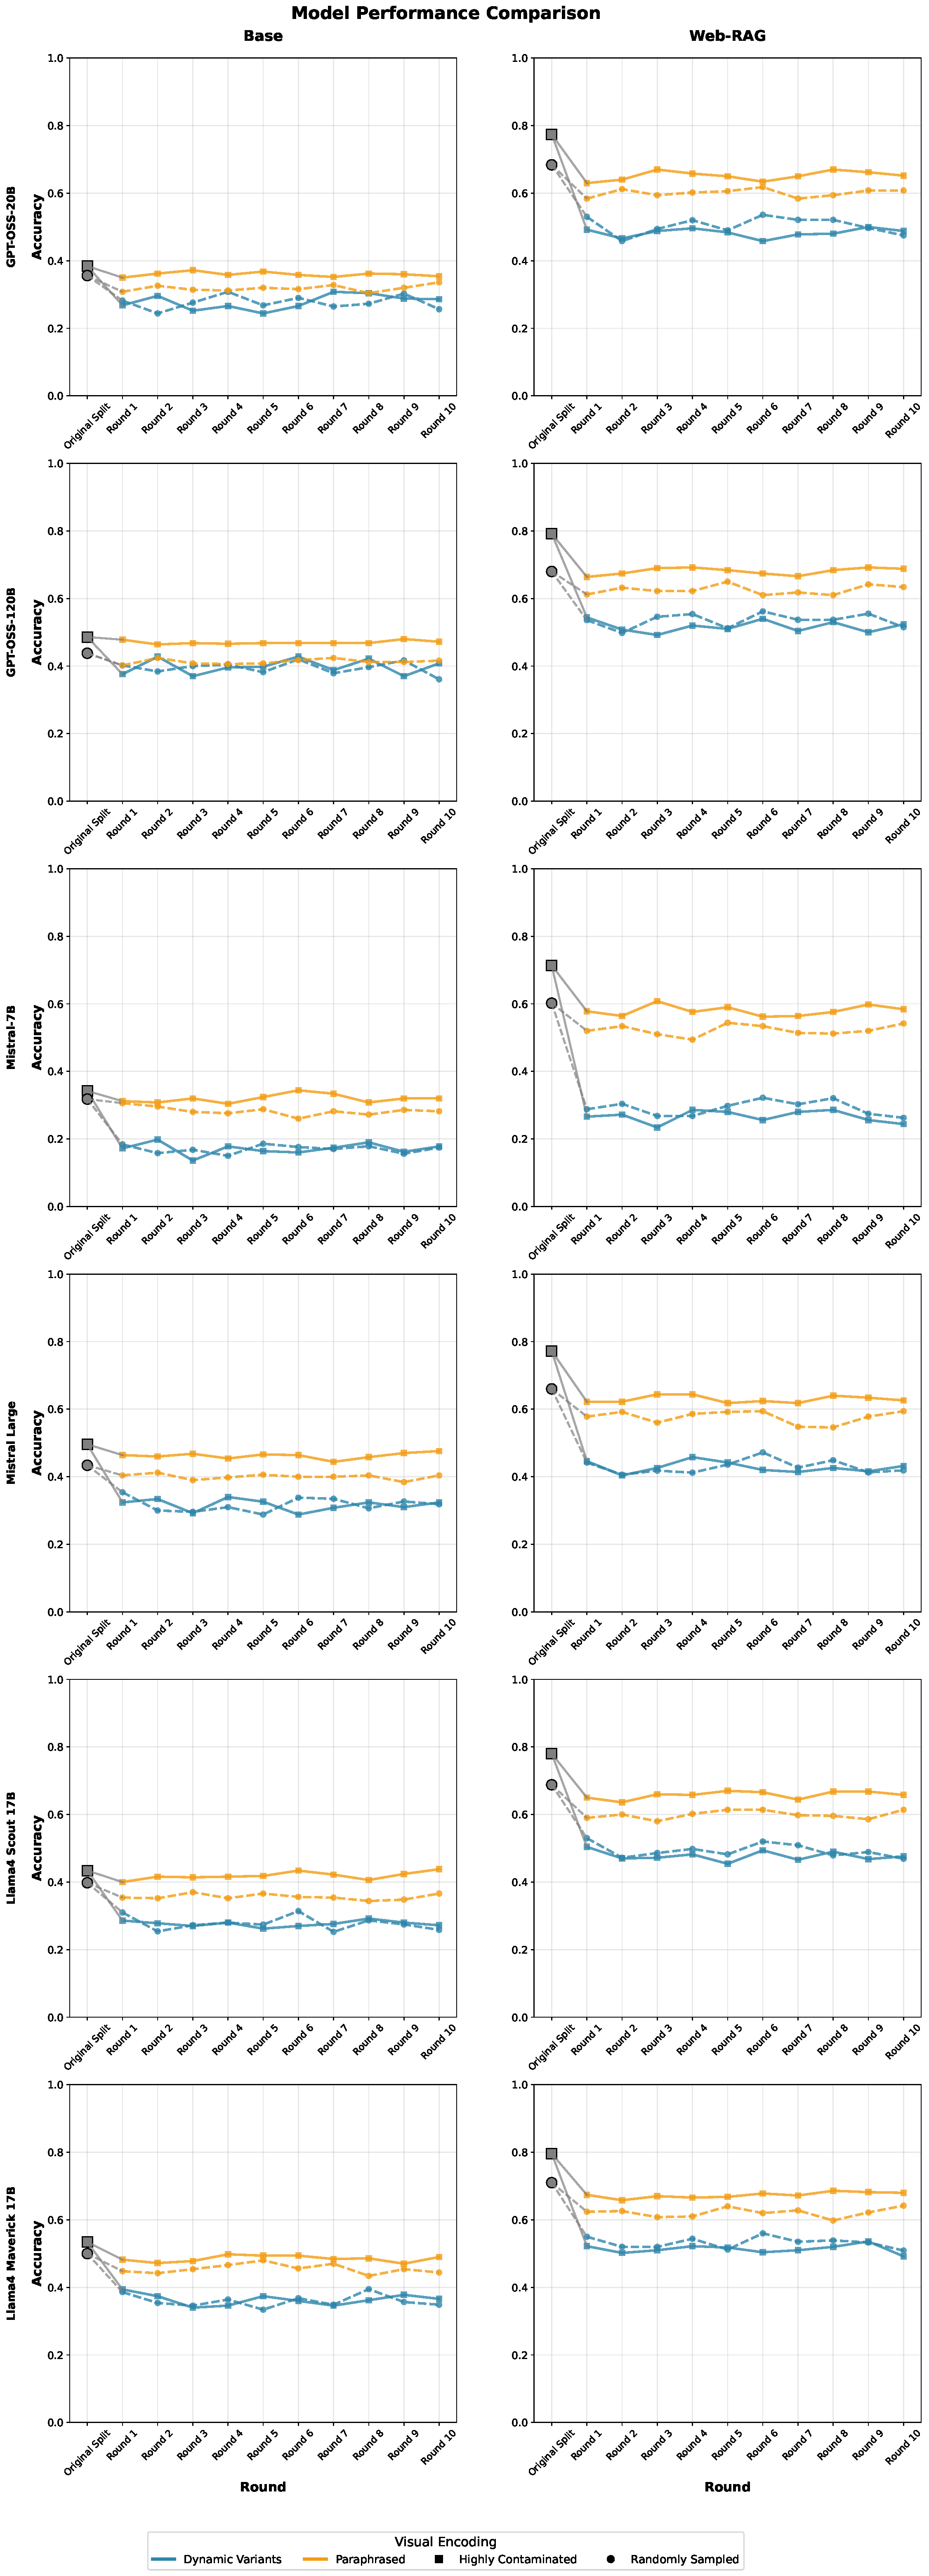
\includegraphics[width=\columnwidth]{res/model_performance_collage.pdf}
    \caption{model\_performance\_collage.pdf}
    \label{fig:model_performance_collage}
\end{figure}

\begin{figure}[htbp]
    \centering
    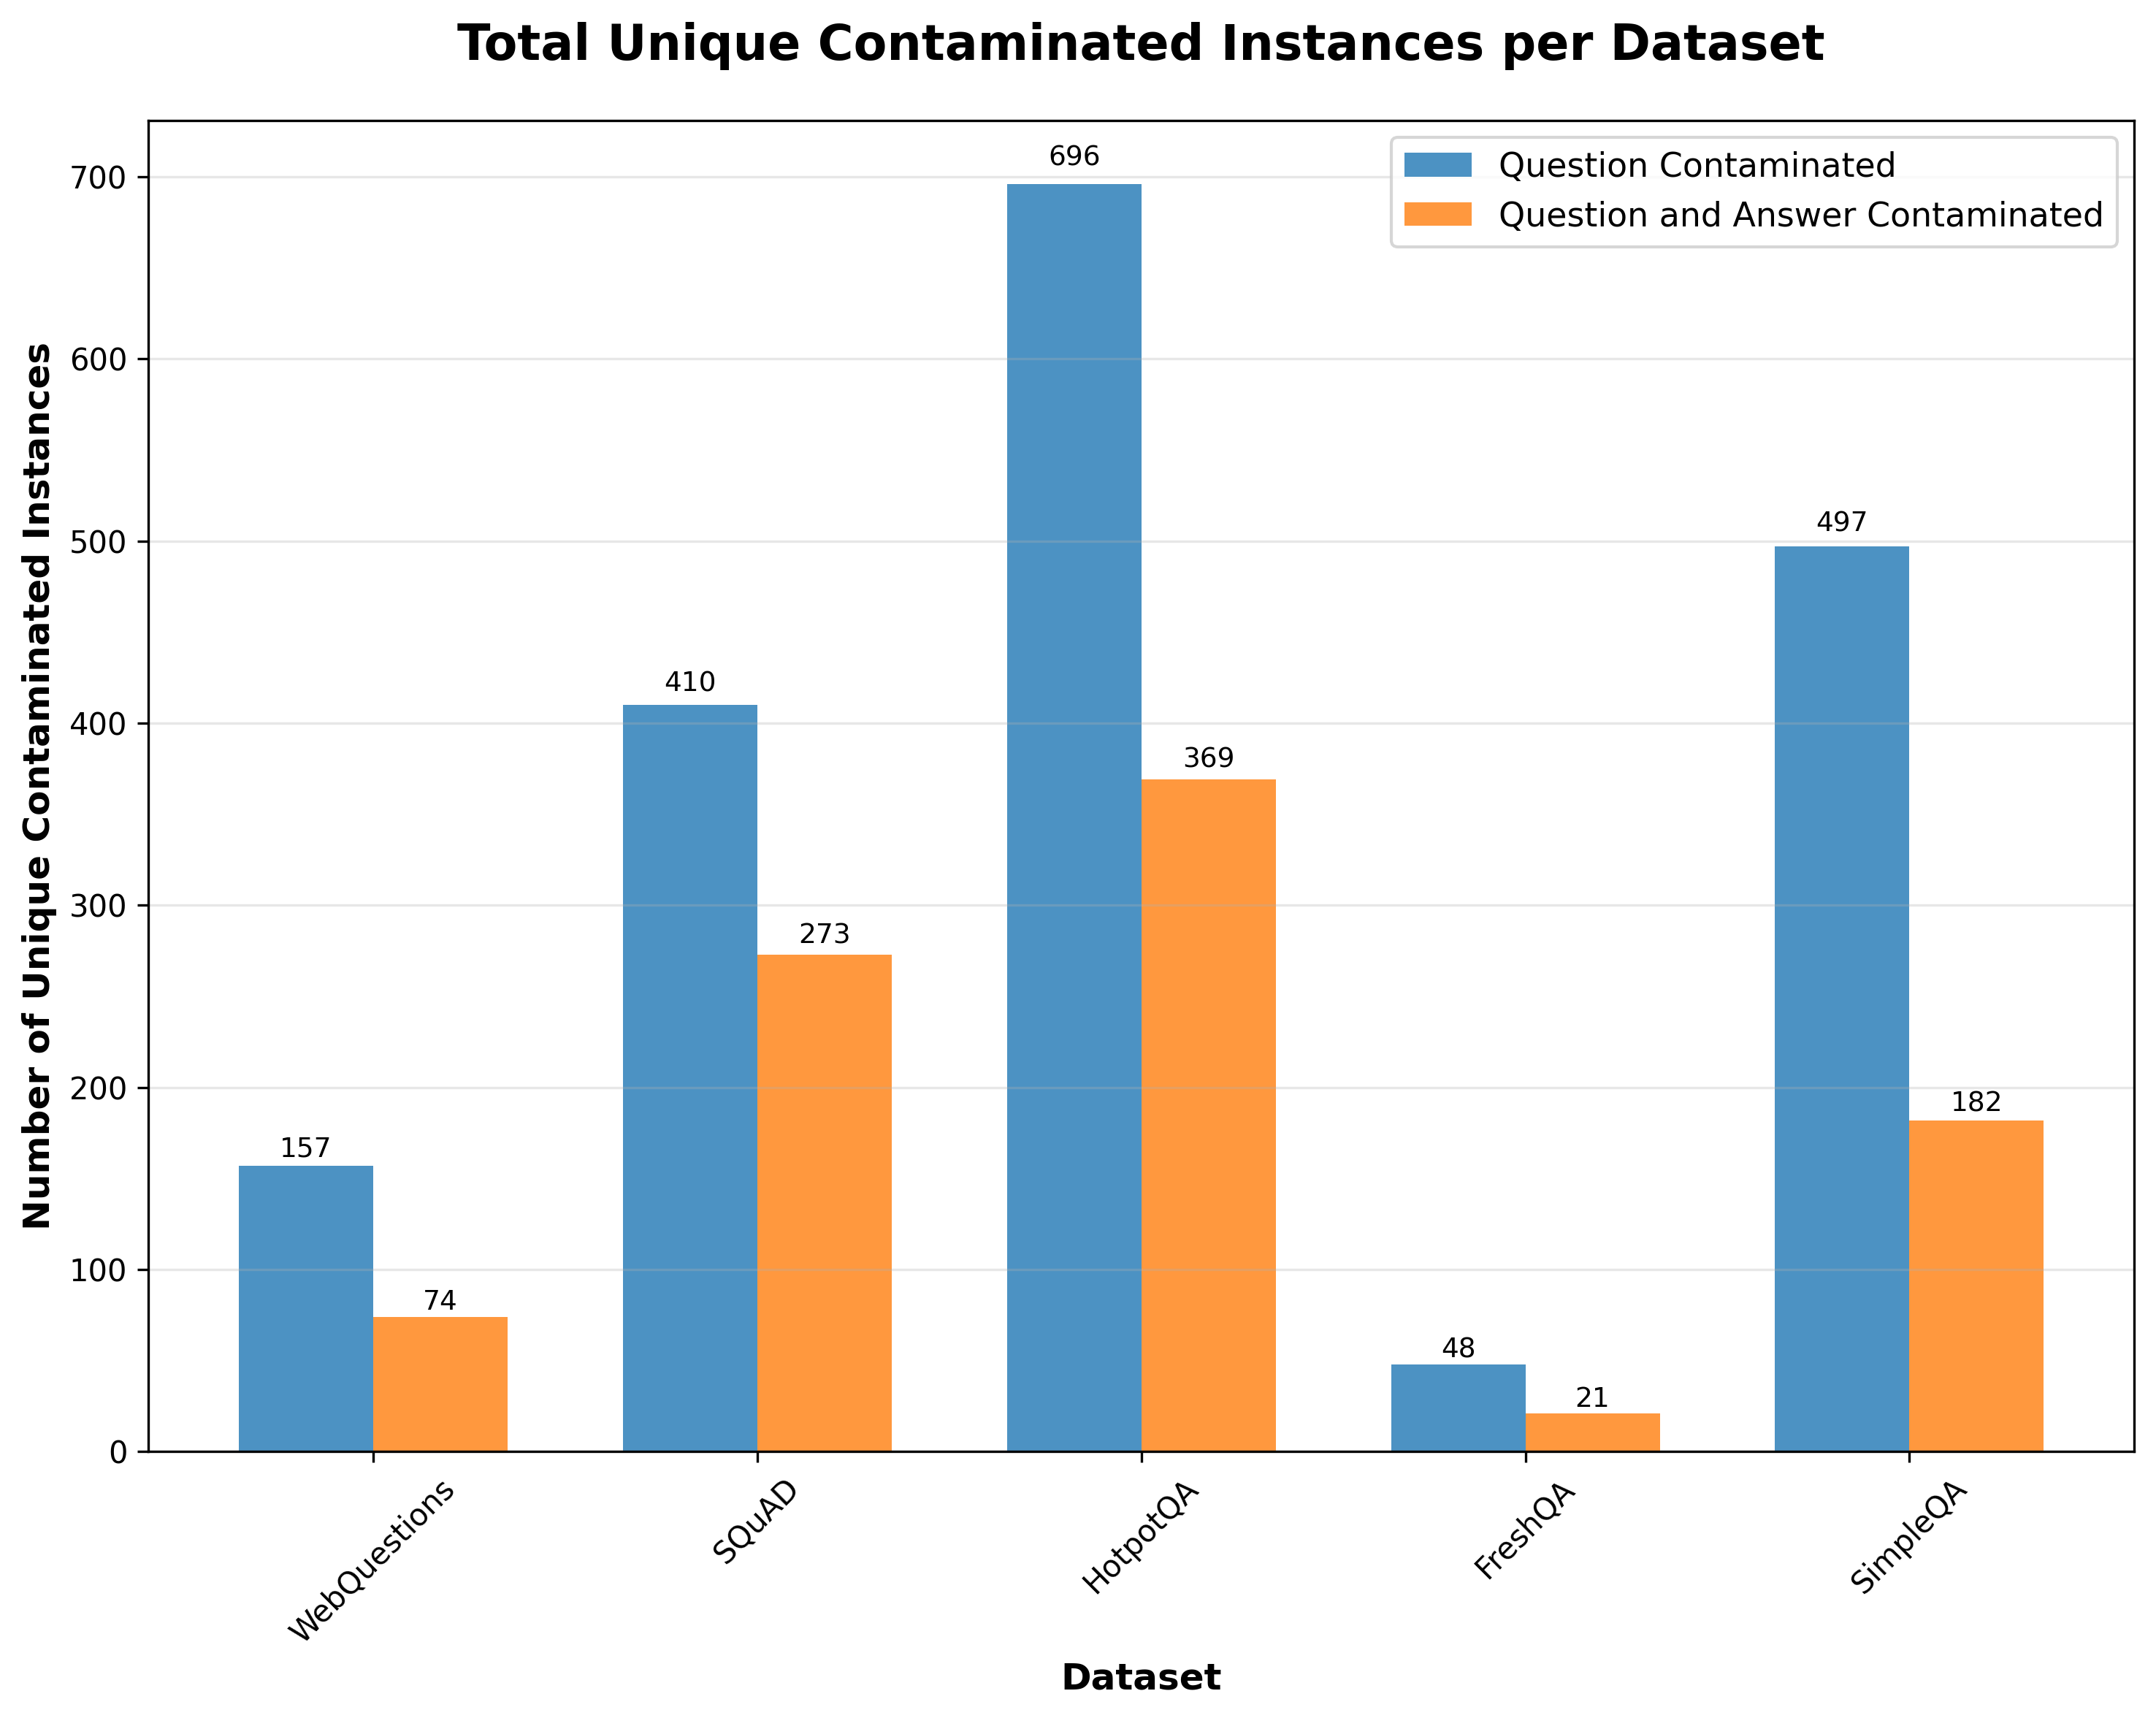
\includegraphics[width=\columnwidth]{res/total_unique_contaminated_instances_per_dataset.png}
    \caption{total\_unique\_contaminated\_instances\_per\_dataset.png}
    \label{fig:total_unique_contaminated_instances}
\end{figure}

\begin{figure}[htbp]
    \centering
    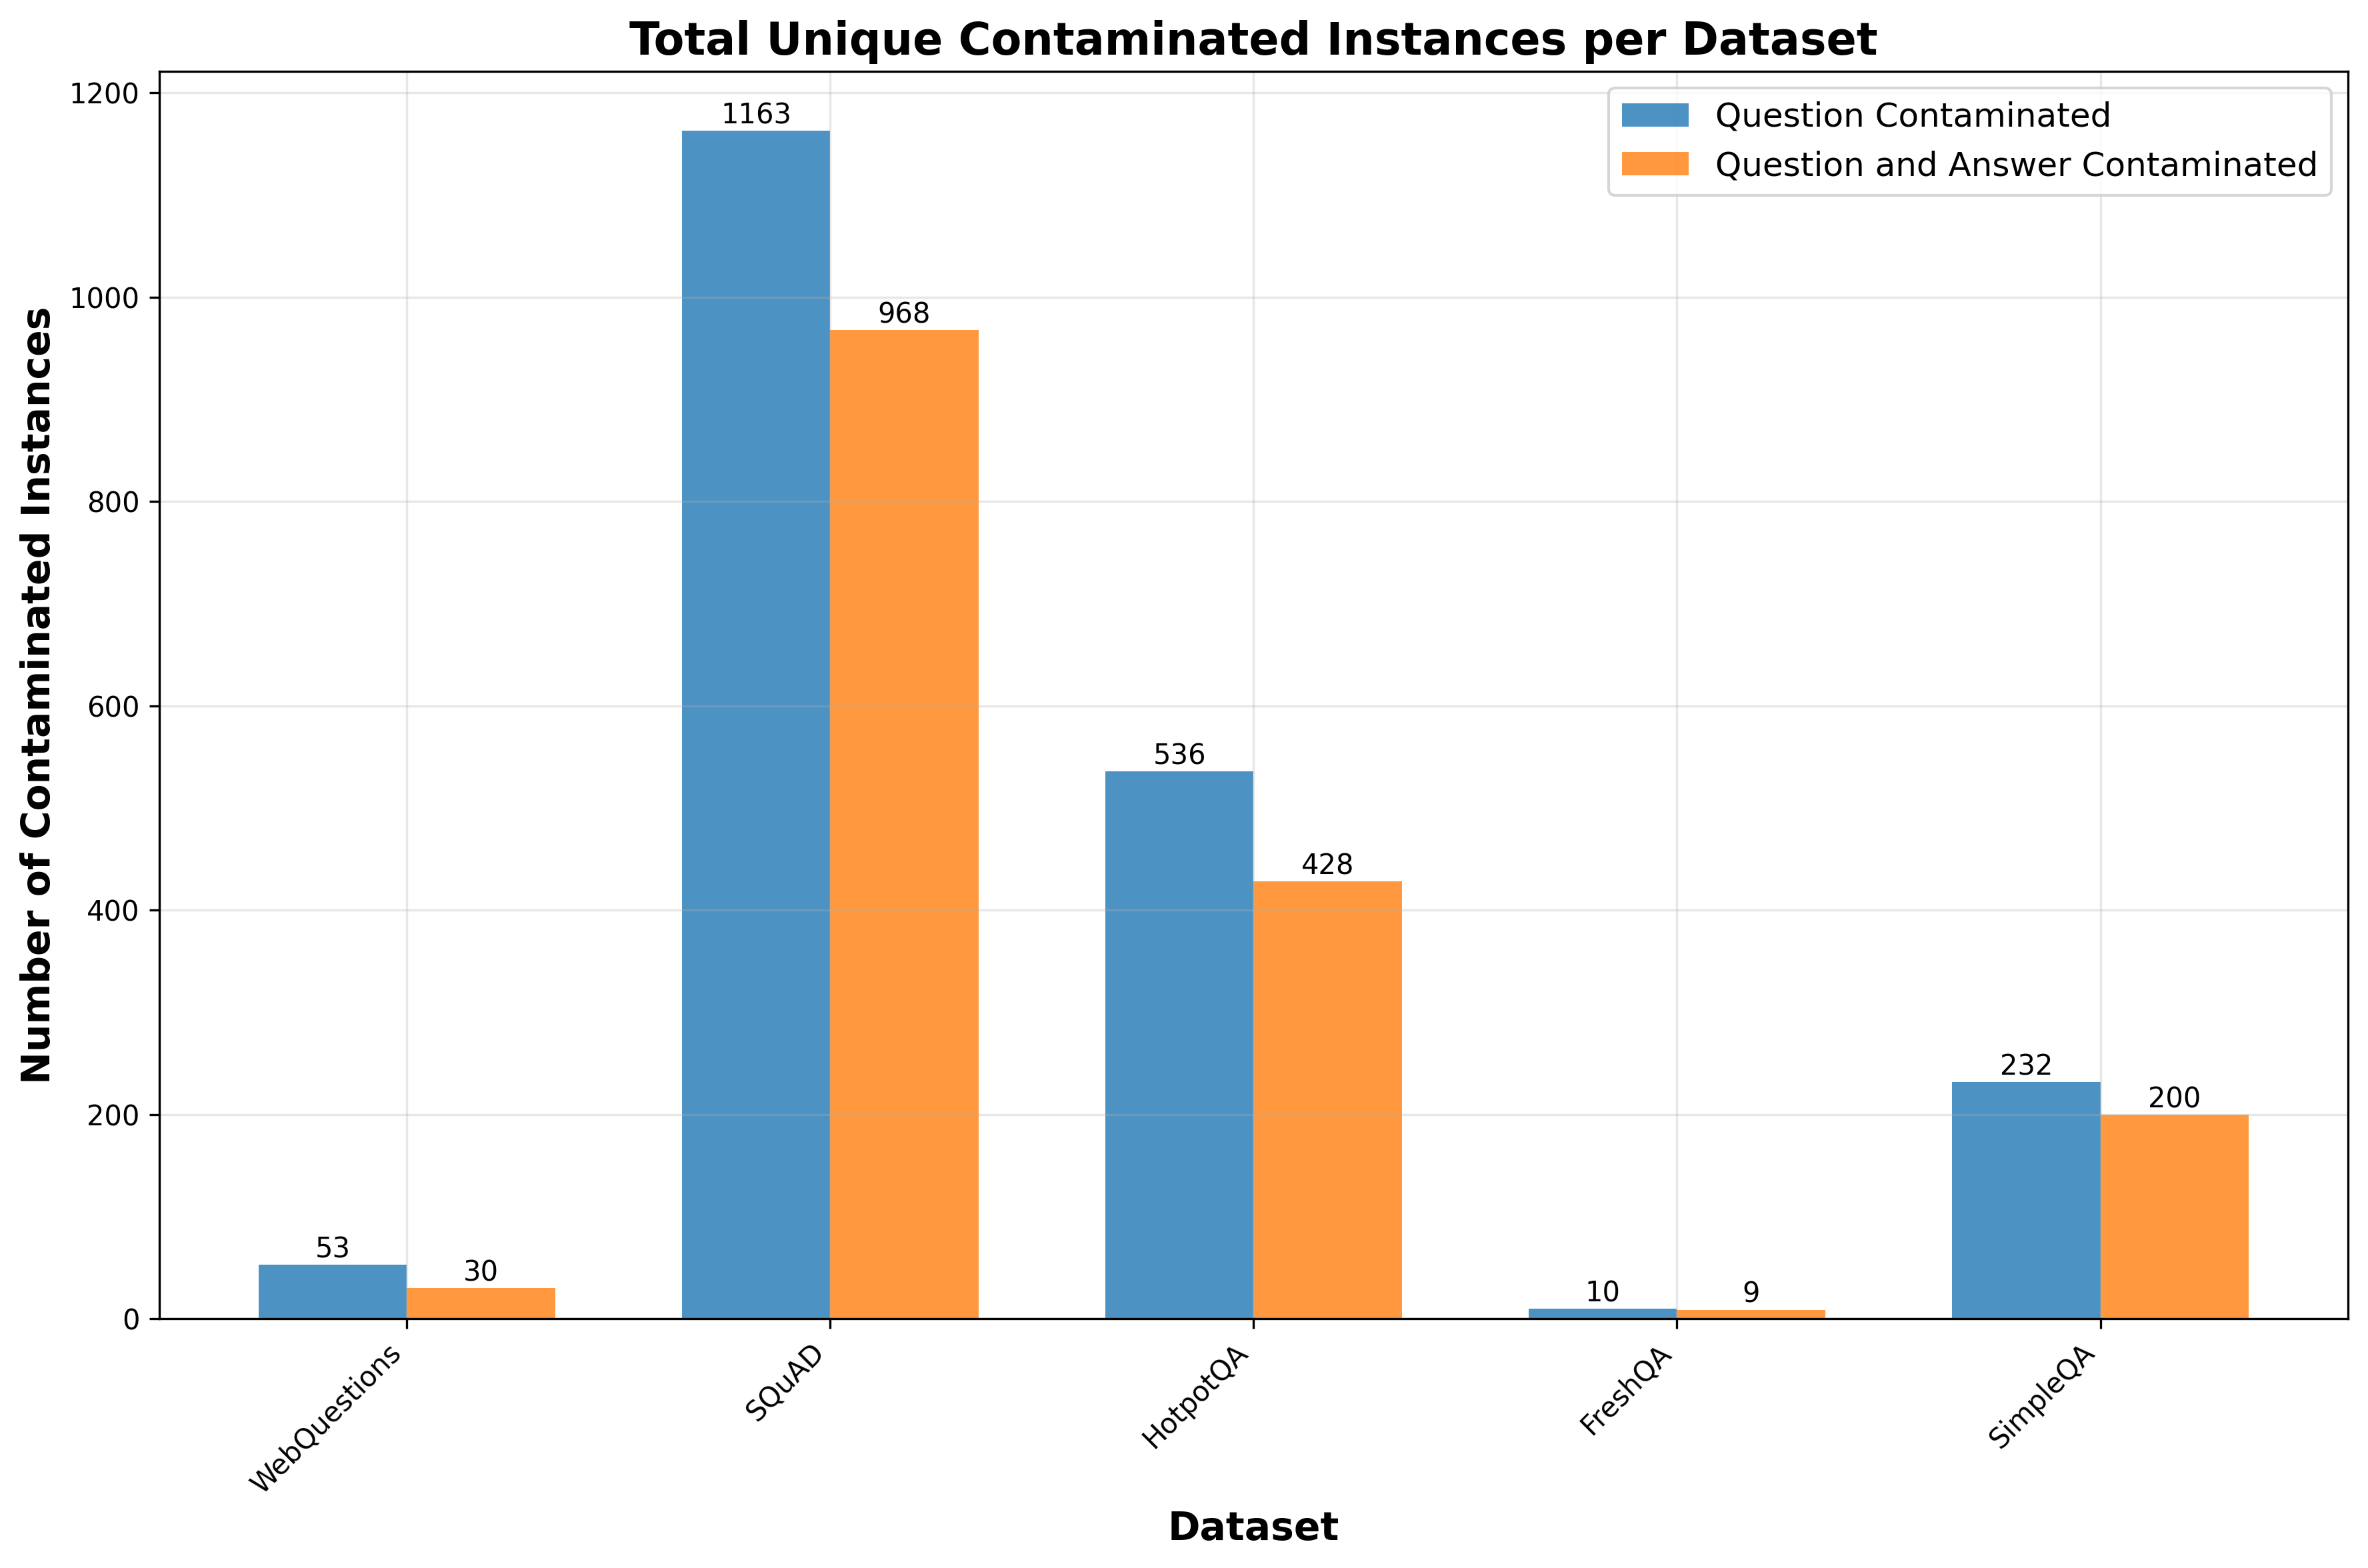
\includegraphics[width=\columnwidth]{res/total_unique_retrieval_contaminated_instances_per_dataset.png}
    \caption{total\_unique\_retrieval\_contaminated\_instances\_per\_dataset.png}
    \label{fig:total_unique_retrieval_contaminated_instances}
\end{figure}

\section{Discussion}
TBD

\section{Conclusion}
TBD


\bibliographystyle{ACM-Reference-Format}
\bibliography{DynamicBenchmarkWebQA}

\end{document}
